% !TEX root = cha-implementation.tex
\documentclass[../../main.tex]{subfiles}

\begin{document}

\section{Wave Function Collapse}

The WFC implementation in \wassis follows the general process described in \secref{sec:soa_wfc}, but introduces some implementation mechanisms to improve the efficiency of the path generation process. This section describes these mechanisms, including heap management, dynamic tile weights, path ID resolution, constraint propagation, and backtracking.

\subsection{Heap Management}
\label{subsec:heap_management}

During the observation phase of WFC, the next cell to collapse is selected as the cell with the highest entropy, as described in \subsecref{subsec:wassis_observation_phase}. Scanning the whole grid at every step would require $O(N)$ time, where $N$ is the total number of cells. To avoid this cost, \wassis uses a max binary heap containing \texttt{WSHeapEntry} objects. The root of the heap contains the cell with the highest entropy, which can be accessed in $O(1)$ time, while removing it requires $O(\log M)$ time, where $M$ is the current size of the heap. The overall process is shown in \figref{fig:heap_workflow}.

\begin{figure}[H]
    \centering
    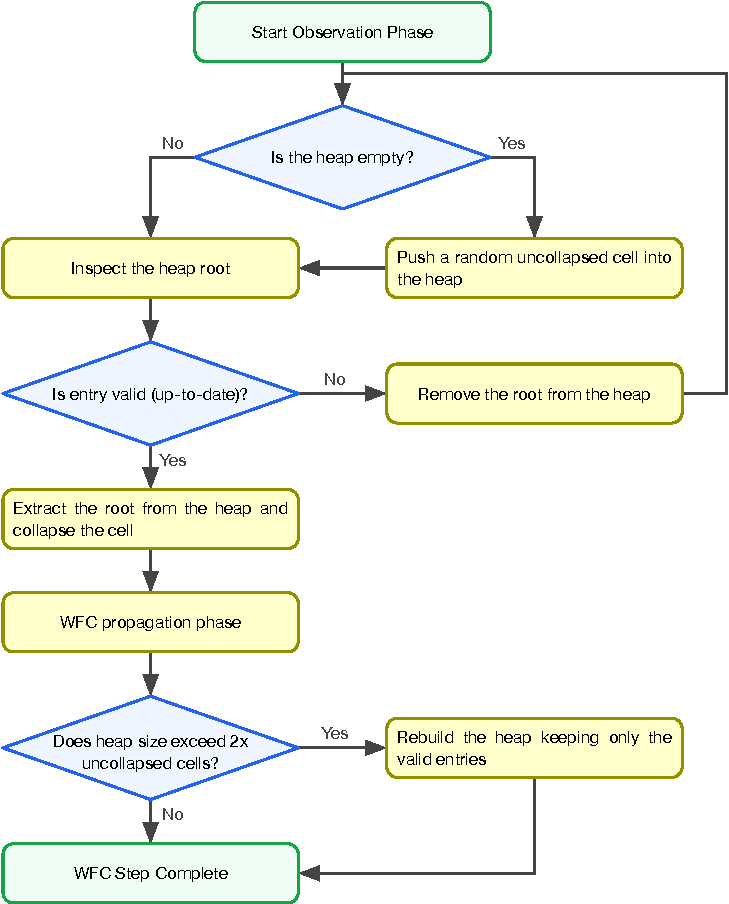
\includegraphics[width=0.89\linewidth]{figures/implementation/heap_workflow}
    \caption{Next cell selection workflow.}
    \label{fig:heap_workflow}
\end{figure}

\paragraph{Initial Insertion}

The heap does not initially contain all grid cells. Only cells occupied by software classes are inserted, as they are the starting points of the WFC generation. Untouched cells are not inserted because initially they all have the same set of possible tiles and therefore the same entropy.

After a propagation step, the cells that were touched by propagation are added to the heap. These cells have fewer possible tiles and therefore a different entropy from untouched cells. Since WFC starts from the class cells and propagation only affects part of the grid at each step, only these cells are added to the heap, keeping its size relatively small.

A cell may be affected multiple times during the same propagation phase. Inserting it into the heap after every change would result in unnecessary operations, especially since propagation is the most computationally intensive parts of WFC. Therefore, affected cells are first collected and inserted into the heap only once, after the propagation phase is complete.

\paragraph{Lazy Heap Entries}

Updating a cell that is already in the heap is expensive with the heap implementation available in Pharo. Finding a specific element inside the heap requires $O(M)$ time. Instead of removing and reinserting a node every time its entropy changes, \wassis uses \texttt{WSHeapEntry} objects.

A \texttt{WSHeapEntry} stores a reference to a \texttt{WSNode}, together with the entropy and the number of possible tiles of that node at the time the entry is created. As a result, more than one entry referring to the same node can exist in the heap. Older entries are not immediately removed when the node changes.

When the root of the heap is selected, the stored values are compared with the current values of the corresponding \texttt{WSNode}. If they do not match, the entry is no longer valid and is removed from the heap in $O(\log M)$ time. The next entry is then checked in the same way until a valid entry is found for collapse.

The number of possible tiles is stored in addition to the entropy because some tiles have weight zero. These tiles do not contribute to the entropy calculation, therefore, entropy alone is not sufficient to determine whether a heap entry represents the current state of a node.

An example of a lazy heap entry is provided in \figref{fig:lazy_entry_example}.

\begin{figure}[H]
    \centering
    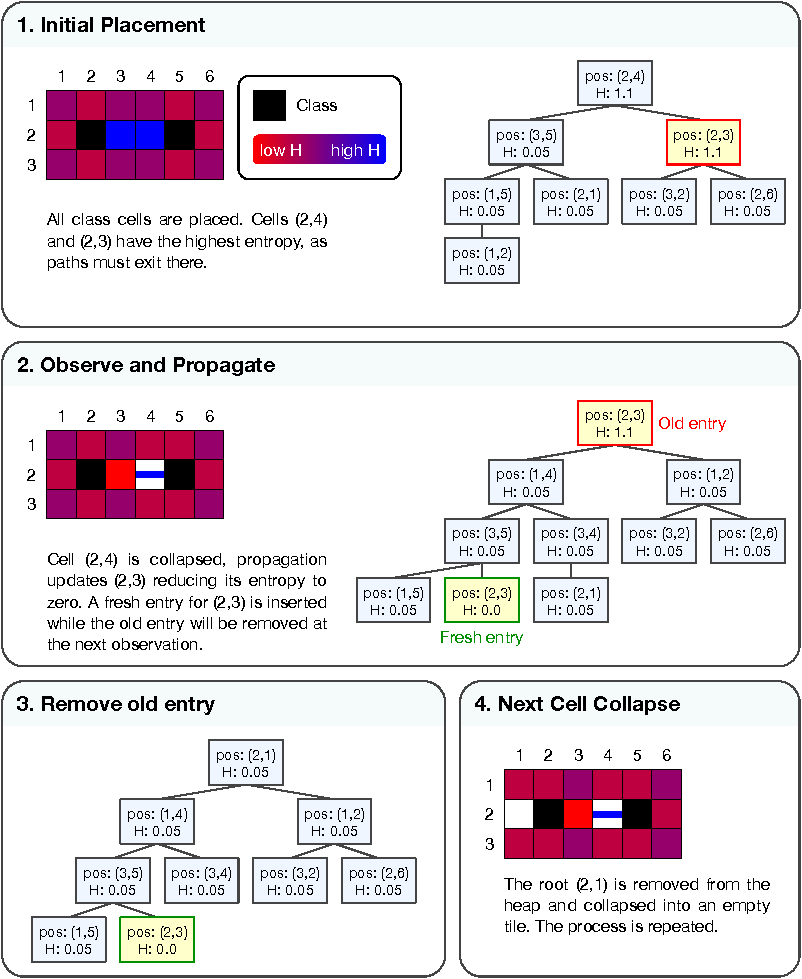
\includegraphics[width=0.862\linewidth]{figures/implementation/lazy_entry_example}
    \caption{Lazy heap entry example.}
    \label{fig:lazy_entry_example}
\end{figure}

\paragraph{Heap Compaction and Empty Heap Handling}

The use of old heap entries means that the heap can contain entries that are no longer valid. To prevent the heap from becoming too large, after each propagation phase \wassis compares the heap size with the number of uncollapsed cells. If the heap has more than double the number of entries respect to the number of uncollapsed cells, it is rebuilt. The rebuild removes old entries and keeps only the current entries of uncollapsed cells.

Finally, because cells are added to the heap only after being touched by propagation, the heap can become empty even though some cells are still uncollapsed. This can happen when the propagation step does not affect any new cell. In this case, a random uncollapsed cell is selected and added to the heap. This is valid because all cells that have never been touched have the same set of possible tiles and therefore the same entropy. The random choice allows the execution to continue until propagation reaches other cells.

\subsection{Dynamic Placeholder Resolution}

A \emph{resolved tile} is a path tile whose edges contain concrete path IDs instead of placeholders. When a node is collapsed to a path tile, \wassis checks its already collapsed neighbors for a resolved path tile. If one is found, its concrete path ID is used to replace the placeholders of the new collapsed tile. If no path ID is available, the tile remains unchanged.

If the new collapsed node is resolved, \wassis then propagates its path ID to already collapsed neighboring nodes containing placeholder tiles. The resolution uses a queue starting from the collapsed node. For each node in the queue, its collapsed neighbors are checked. If a neighbor contains a placeholder tile and its path ID can be determined from the current node, the placeholder is replaced with a concrete tile. Successfully resolved nodes are added to the queue so that the path ID can continue to propagate through adjacent collapsed nodes.

After this resolution process, \wassis checks the edges of the resolved tiles against their collapsed neighbors. If two adjacent resolved tiles have incompatible edges, a contradiction is signaled.

\subsection{Dynamic Tile Weights}

To guide paths toward their targets, \wassis uses dynamic tile weights in addition to fixed path exits. When a cell is selected for collapse, its possible tiles are assigned weights based on the direction of the target for the weighted choice. If the cell has a path target, \wassis increases the weight of tiles whose shape point toward that target.

Path target information is propagated in the same way as path IDs. Initially, target information is associated with the classes placed on the grid. When a path ID is propagated to a resolved path tile, the corresponding target information is also propagated. This allows cells along the path to know the target associated with the path they will collapse to.

On a 2D grid, \wassis compares the position of the current cell with the position of the target along the two axes. The distance along each axis is used to determine which directions lead to the target. The boost per direction depends on how much of the remaining distance is along that axis.

As illustrated in \figref{fig:boosted_tile}, if the current cell is at position $(4,4)$ and the target is at position $(2,7)$, the remaining distance is $2$ cells along the vertical axis and $3$ cells along the horizontal axis, for a total of $5$. Therefore, the horizontal direction receives a larger boost than the vertical direction. The boost is controlled by a value chosen by the user. For example, with a boost value of $10$, the vertical direction receives a factor of $10 \cdot \frac{2}{5} = 4.0$, while the horizontal direction receives a factor of $10 \cdot \frac{3}{5} = 6.0$. If a tile has an original weight of $2$ and points in the horizontal direction, its new weight becomes $2 \cdot 6.0 = 12.0$. If boost is $0$ the tile keeps its original weight. Zero-weight tiles are unaffected by the boost.

When a tile can help guide the same path in more than one direction, only the highest boost is used. For example, if a tile points both vertically and horizontally toward a target, with boost factors of $4.0$ and $6.0$ respectively, the tile receives a boost of $6.0$. This prevents the tile from receiving a too large boost just because it has multiple useful directions for the same path.

If a tile can help guide multiple paths, the highest boost is selected for each path. These boosts are then multiplied together. The original tile weight is multiplied by the resulting value. This makes tiles that help guide multiple paths more likely to be selected.

\begin{figure}[ht]
    \centering
    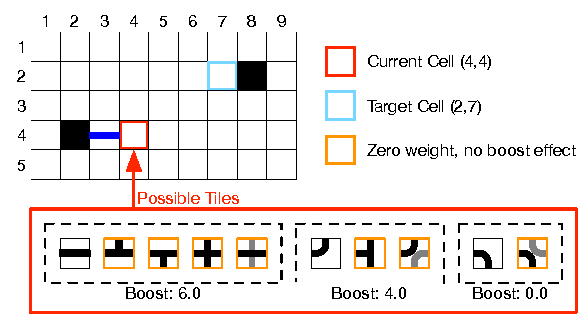
\includegraphics[width=\linewidth]{figures/implementation/boosted_tile}
    \caption{Example of tile weight boost.}
    \label{fig:boosted_tile}
\end{figure}

\subsection{Constraint Propagation}

After the collapse of a node and the path ID resolution step, constraint propagation is performed. First, propagation starts from the new collapsed node and uses a FIFO queue. The initial node is added to the queue, and nodes are processed until the queue is empty. For each node, its neighbors are examined. Already collapsed neighbors are skipped, since their tile is already fixed and cannot be changed. For each uncollapsed neighbor, the possible tiles are reduced according to the current constraints. A tile is kept only if the symbol on its edge facing the current node is compatible with the corresponding symbol of the tile selected for the current node.

If one or more tiles are removed from a neighbor, its entropy is updated and the neighbor is added to the queue so that the updated constraints can be propagated recursively to its neighbors.

If a neighbor loses all its possible tiles, a contradiction is detected and the backtracking process described in \subsecref{subsec:backtracking_strategies} starts.

The propagation process keeps track of all nodes whose possible tiles have changed. Once the queue is empty, these nodes are used to update the max-heap described in \subsecref{subsec:heap_management}. Updating the heap only once at the end of propagation avoids repeated heap operations if the same node is affected multiple times during the same propagation step.

\subsection{Backtracking}
To make backtracking possible, the state of the grid must be saved at different points during the generation. The \texttt{WSBacktracking} class decides when to create a checkpoint depending on the selected backtracking strategy. The checkpoint is evaluated after a cell has been selected for collapse but before a tile is actually chosen. This allows the checkpoint to represent the exact state from which the current decision is made. If the decision later leads to a contradiction, the state can be restored and the tile originally selected at that decision point can be removed from the cell's possible tiles before collapsing it again.

The initial implementation used a deep copy of the \texttt{WSGraph} object. However, this was very expensive and had a significant impact on performance. To avoid copying the entire object, the Memento pattern was used. The \texttt{WSGraph} and \texttt{WSNode} classes provide methods to create snapshots of their current state, represented by \texttt{WSGraphSnapshot} and \texttt{WSNodeSnapshot}. These snapshots store only the mutable state needed to restore the current state. A \texttt{WSGraphSnapshot} contains the snapshots of its nodes and a copy of the heap, reducing the cost of saving checkpoints.  \clearpage  It is then stored in a \texttt{WSCheckpoint} along with other information (\eg a timestamp), while \texttt{WSBacktracking} keeps the collection of available checkpoints.

When a checkpoint has to be restored, \texttt{WSBacktracking} asks the \texttt{WSGraph} to restore its state from the corresponding snapshot. This approach avoids the expensive deep copy of the whole graph and improves performance at the cost of additional memory for the stored snapshots.

While the other backtracking strategies are relatively simple to evaluate, the \emph{similar weights} strategy requires a more complex check. With the fixed and percentage strategies, a checkpoint is created at every step. The \emph{many possible tiles} strategy only requires checking whether the number of possible tiles is above the selected threshold, while \emph{restart} strategy does not create checkpoints.

The \emph{similar weights} strategy instead requires checking whether a sufficient number of possible tiles have similar weights. The user defines the minimum percentage of tiles that must have similar weights and the maximum allowed difference between their weights, also expressed as a percentage.

To perform this check, tiles with zero weight are first ignored and the remaining weights are sorted. A sliding window is then used to examine groups of the required size. For each group, the difference between the smallest and largest weight is compared with the allowed difference. If at least one group satisfies this condition, a checkpoint is created. The sliding window allows all groups of the required size to be checked efficiently after sorting the weights.

\end{document}